\chapter{TBD}

\section{Elliptic Systems}
\underline{Some info abput existence of weak solutions}

We consider functions \(u: \Omega \subset \mathbb{R}^{n} \to \mathbb{R}^{m}\). We use Greek letters to indicate components of vectors in the starting domain (so that \(\alpha,\beta \in \{1,2,\dots,n\} \)) and we use latin letters to indicate components of vectors in teh target domain (so that \(i.j \in \{1,2,\dots,n\} \)). Furthermore, we work with matrices with 4 indices (rank-four tensors). As usually done for elliptic equations we will define ellipticity as the positive semi-definiteness of the tensor, namely the Legendre condition~\eqref{E} below:
\begin{gather}
	\exists c > 0 : \sum_{\alpha,\beta,i,j} A_{ij}^{\alpha\beta} \xi_{\alpha}^{i} \xi_{\beta}^{j} \geq c \abs{\xi}^{2}, \forall \xi \in \mathbb{R}^{m \times n} \tag{E}\label{E}
\end{gather}
We can employ the condition~\eqref{E} to prove existence and uniqueness results for
\begin{gather}
	\begin{cases}
		- \sum_{\alpha, \beta, j} \partial_{x_\alpha} (A_{ij}^{\alpha \beta} \partial_{x_{\beta}} u^{j}) = f_{i} - \sum_{\alpha}^{} \partial_{x_{\alpha}} F_{i}^{\alpha}\qquad i=1,\dots,m \\
		u \in H_{0}^{1}(\Omega; \mathbb{R}^{m})
	\end{cases} \tag{LS}\label{LS}
\end{gather}
with data \(f_{i},F_{i}^{\alpha} \in L^{2}(\Omega;\mathbb{R})\).\\
The weak formulation of the problem is readily obtained as
\begin{gather}
	\int\limits_{\Omega}^{} \sum_{\alpha, \beta, i,j}^{} A_{ij}^{\alpha \beta} \partial_{x_{\beta}} u^{i} \partial_{x_{\alpha}} \phi^{i} \dd{x} = \int\limits_{\Omega}^{} \Big[f_{i} \phi^{i} + \sum_{\alpha,i}^{} F_{i}^{\alpha} \partial_{x_{\alpha}} \phi^{i} \Big] \dd{x} \qquad \forall \phi \in C_c^\infty(\Omega;\mathbb{R}^{m})
\end{gather}
The matrix \(A_{ij}^{\alpha \beta}\) defines a bilinear continuous form on \(H_0^1(\Omega;\mathbb{R}^{m})\) by means of the formula
\begin{gather}
	{(\phi,\psi)}_A := \int\limits_{\Omega}^{} \sum_{\alpha, \beta, i,j}^{} A_{ij}^{\alpha \beta} \partial_{x_{\alpha}} \phi^{i} \partial_{x_{\beta}} \psi^{j} \dd{x}
\end{gather}
If moreover \(A_{ij}^{\alpha \beta}\) satisfies the Legendre condition~\eqref{E}, then the bilinear form is coercive, and we can use the Lax-Milgram theorem to prove existence and uniqueness of weak solutions. Actually one can prove existence and uniqueness under a weaker assumption known as \enquote{Legendre-Hademard}~\eqref{LH} condition:
\begin{gather}
	\sum_{\alpha,\beta,i,j}^{} A_{ij}^{\alpha \beta} \xi_{\alpha}^{i} \xi_{\beta}^{j}\geq \lambda \abs{\xi}^{2} \qquad \forall \xi=a \otimes b \tag{LH} \label{LH}
\end{gather}
that is the Legendre condition~\eqref{E} for rank-one matrices \(\xi=a\otimes b\).\\
The~\eqref{LH} condition is strictly weaker than~\eqref{E}, as the following example shows.

\begin{exm}[\eqref{LH} is weaker than~\eqref{E}]
	Let \(m=n=2\) and let \(A_{ij}^{\alpha \beta}\) be such that
	\begin{gather}
		\sum_{\alpha, \beta, i,j}^{}  A_{ij}^{\alpha \beta} \xi_{\alpha}^{i} \xi_{\beta}^{j} = \det{\xi} + \epsilon \abs{\xi}^{2}
	\end{gather}
	for some \(\epsilon \geq 0\) to be chosen later.\\
	Since any rank-one matrix \(\xi = a \otimes b\) has \(\det{\xi}=0\), the~\eqref{LH} condition is fulfilled with \(\lambda = \epsilon \). On the other hand for \(\overline{\xi} = \diag(t,-t), t \neq 0\), we get
	\begin{gather}
		\sum_{\alpha, \beta, i,j}^{}  A_{ij}^{\alpha \beta} \overline{\xi}_{\alpha}^{i} \overline{\xi}_{\beta}^{j} = \det{\overline{\xi}} + \epsilon \abs{\overline{\xi}}^{2} = -t^{2}+2 \epsilon t^{2} = t^{2}(2 \epsilon -1)
	\end{gather}
	and the Legendre condition~\eqref{E} fails for \(2 \epsilon-1 <0\).
\end{exm}
Nevertheless, the following \underline{Theorem} by G\r{a}rding holds true:
\begin{thm}
	Assume that the constant matrix \(A_{ij}^{\alpha \beta}\) satisfies the Legendre-Hademard~\eqref{LH} condition for some positive constant \(\lambda \). Then there exists a unique solution of the linear system~\eqref{LS}.
\end{thm}

\section{Classical regularity theory for the linear problems}
We want to study the local behavior of the weak solutions \(u \in H_{loc}^{1}(\Omega; \mathbb{R}^{m})\) of a system of equations given by:
\begin{gather}
	- \sum_{\alpha, \beta, j} \partial_{x_\alpha} (A_{ij}^{\alpha \beta} \partial_{x_{\beta}} u^{j}) = f_{i} - \sum_{\alpha}^{} \partial_{x_{\alpha}} F_{i}^{\alpha}\qquad i=1,\dots,m
\end{gather}
with \(A_{ij}^{\alpha \beta} \in L^{\infty}(\Omega;\mathbb{R}), f_{i}\in L^{2}_{loc}(\Omega;\mathbb{R}), F_{i}^{\alpha}\in L_{loc}^{2}(\Omega;\mathbb{R})\).\\
In what follows we will always assume \(\Omega \subset \mathbb{R}^{m}\) to be an open, bounded and regular domain (here \(\Omega \) regular means that \(\Omega \) is locally the epigraph of a \(C^{1}\) function of \((n-1)\)-variables, written in a suitable system of coordinates, near any boundary point).\\
We will see how to use a Caccioppoli-Leray inequality to prove existence of higher-order weak derivatives of \(u\) and suitable integrability results thereof. We will moreover turn such estimates into actual regularity results thanks to Sobolev embeddings. The idea above is due L. Nirenberg.\\
We use the symbol \(\abs{\cdot}\) to denote the Hilbert-Schmidt norm of matrices and tensors, even though some estimates would be true also for the smaller operator norm.
We set
\begin{gather}
	\abs{A_{ij}^{\alpha \beta}}^{2} = \sum_{\alpha, \beta, j}  {(A_{ij}^{\alpha \beta})}^{2}
\end{gather}

\begin{thm}[Caccioppoli-Leray inequality]
	If the Borel coefficients \(A_{ij}^{\alpha \beta}\) satisfy the Legendre condition with \(\lambda>0\), namely
	\begin{gather}
		\sum_{\alpha,\beta,i,j} A_{ij}^{\alpha\beta} \xi_{\alpha}^{i} \xi_{\beta}^{j} \geq \lambda \abs{\xi}^{2}, \forall \xi \in \mathbb{R}^{m \times n}
	\end{gather}
	and
	\begin{gather}
		\sup_{x \in \Omega} \abs{A_{ij}^{\alpha\beta}(x)} \leq \Lambda < + \infty
	\end{gather}
	then there exists a positive constant \(C_{CL} = C_{CL}(\lambda, \Lambda)\) such that, for any ball \(B_{R}(x_{0})\subset \subset \Omega \) and any \(k \in \mathbb{R}^{m}\) it holds
	\begin{gather}
		C_{CL}\int\limits_{B_{\sfrac{R}{2}}(x_{0})}^{} \abs{\nabla u}^{2} \dd{x} \leq R^{-2}\int\limits_{B_{R}(x_{0})}^{} \abs{u(x)-k}^{2} \dd{x} + R^{2}\int\limits_{B_{R}(x_{0})} \abs{f(x)}^{2} \dd{x} +  \int\limits_{B_{R}(x_{0})} \abs{F(x)}^{2} \dd{x} \tag{CLI}\label{CLI}
	\end{gather}
\end{thm}
\begin{remark}
	\begin{itemize}
		\item the validity of~\eqref{CLI} on all \(k \in \mathbb{R}^{m}\) depends on the fact that the PDE is invariant under translation of \(u\), meaning that if \(u\) is a solution, then also \(u+k\) \(\forall k\) is a solution
		\item note also that the inequality is scale invariant: think about \(u\) being adimensional, then all the terms in~\eqref{CLI} have dimension \({(\text{length})}^{n-2}\)
		\item the inequality is surely non-trivial (the gradient of a function cannot be controlled by the variation of the function!).~\eqref{CLI} can already be regarded as a first regularity result, meaning that we are gaining specific information on the behavior of a function from the fact that it is a solution of a PDE
	\end{itemize}
\end{remark}
\begin{proof}
	W.l.o.g we take \(x_{0}=0\) and \(k=0\). We choose as test function \(\phi \) in the weak formulation
	\begin{gather}
		\int\limits_{B_{R}}^{} \left\langle  A \nabla u, \nabla \phi \right\rangle \dd{x} - \int\limits_{B_{R}}^{} \left\langle  f,\phi \right\rangle \dd{x} -\int\limits_{B_{R}}^{} \left\langle  F,\nabla\phi \right\rangle \dd{x} =0
	\end{gather}
	the function \(\phi:= u \eta^{2}\), where \(\eta \in C_{c}^{\infty}(B_{R}; \mathbb{R})\) is a cut-off function with \(\eta \equiv 1\) in \(B_{\sfrac{R}{2}}\), \(0 \leq \eta \leq 1\) and \(\norm{\nabla \eta}_{\infty} \leq \frac{4}{R}\)
	\begin{center}
		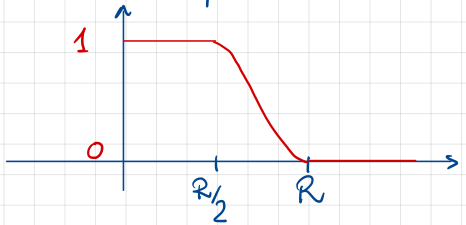
\includegraphics[scale=0.45]{pictures/picture01.png}
	\end{center}
	\begin{gather}
		\pdv[]{\phi_{i}}{x_{\alpha}} = \pdv[]{}{x_{\alpha}} (\eta^{2}u^{2}) = \eta^{2}\pdv[]{u^{i}}{x_{\alpha}}+2 \eta \pdv[]{\eta}{x_{\alpha}} u^{i},
	\end{gather}
	that is
	\begin{gather}
		\nabla \phi = \eta^{2} \nabla u + 2 \eta u \otimes \nabla \eta.
	\end{gather}
	Plugging in the last equality in the weak formulation
	\begin{align}
		0= & \int\limits_{B_{R}}^{} \eta^{2} \left\langle A \nabla u , \nabla u \right\rangle + 2 \int\limits_{B_{R}}^{} \eta \left\langle A \nabla u , u \otimes \nabla \eta \right\rangle  \\
		   & - \int\limits_{B_{R}}^{} \eta^{2} \left\langle f, u \right\rangle - \int\limits_{B_{R}}^{} \eta^{2} \left\langle F, \nabla u \right\rangle - 2 \int\limits_{B_{R}}^{} \eta \left\langle  F, u \otimes \nabla \eta \right\rangle  \\
		=  & : I_{1} + I_{2} -I_{3} - I_{4} - I_{5}
	\end{align}
	\begin{align}
		I_{1}:= & \int\limits_{B_{R}}^{} \eta^{2} \left\langle A \nabla u , \nabla u \right\rangle \dd{x}
		= \int\limits_{B_{R}}^{} \sum_{\alpha, \beta, i, j} \eta^{2} A_{ij}^{\alpha \beta} \partial_{x_{\alpha}} u^{i} \partial_{x_{\beta}} u^{j} \dd{x} \geq \lambda \int\limits_{B_{R}} \eta^{2} \abs{\nabla u}^{2}  \dd{x}  \\
		I_{2}:= & \, 2 \int\limits_{B_{R}}^{} \eta \left\langle A \nabla u , u \otimes \nabla \eta \right\rangle \dd{x} = 2 \int\limits_{B_{R}}^{} \eta \sum_{\alpha,\beta, i, j} A_{ij}^{\alpha \beta} \partial_{x_{\alpha}} u^{i} u^{j} \partial_{x_{\beta}} \eta \dd{x}  \\
		        & \overset{\text{Cauchy-Schwarz}}{\leq} 2 \int\limits_{B_{R}}^{} \eta \abs{A} \abs{u}\abs{\nabla u}\abs{\nabla \eta} \dd{x}  \\
		        & \overset{\text{boundedness of \(\abs{A}\) and \(\norm{\nabla \eta}_{\infty}\)}}{\leq}   \frac{( \Lambda)}{R} \int\limits_{B_{R}}^{} (\eta \abs{\nabla u}) \abs{u} \dd{x}  \\
		        & \overset{\text{Young \(ab \leq \frac{a^{2}}{2}+\frac{b^{2}}{2}\)}}{\leq} \frac{4 \Lambda}{R} \epsilon \int\limits_{B_{R}}^{} \eta^{2} \abs{\nabla u}^{2} \dd{x} + \frac{4 \Lambda}{R \epsilon} \int\limits_{B_{R}}^{} \abs{u}^{2} \dd{x}  \\
		I_{3}:= & \int\limits_{B_{R}}^{} \left\langle f, \eta^{2} u \right\rangle \dd{x} = \int\limits_{B_{R}}^{} \eta^{2} \sum_{i}^{} f_{i}u^{i} \dd{x}
		\overset{Young}{\leq} \frac{1}{2 R^{2}} \int\limits_{B_{R}}^{} \abs{u}^{2} \dd{x} + \frac{R^{2}}{2} \int\limits_{B_{R}}^{} \abs{f}^{2} \dd{x}  \\
		I_{4}:= & \int\limits_{B_{R}}^{} \eta^{2} \left\langle F, \nabla u \right\rangle \dd{x} = \int\limits_{B_{R}}^{} \eta^{2}\sum_{\alpha,i}^{} F_{i}^{\alpha} \partial_{x_{\alpha}} u^{i} \dd{x}
		\leq \frac{\lambda}{4} \int\limits_{B_{R}}^{} \eta^{2} \abs{\nabla u}^{2} \dd{x} + \frac{1}{\lambda} \int\limits_{B_{R}}^{} \abs{F}^{2} \dd{x}
		\intertext{By Cauchy-Schwarz inequality, \(\norm{\nabla \eta}_{\infty} \leq \frac{4}{R}\) and Young inequality we have}
		I_{5}:= & \, 2 \int\limits_{B_{R}}^{} \eta \left\langle F, u \otimes \nabla \eta \right\rangle \dd{x} = 2 \int\limits_{B_{R}}^{} \sum_{\alpha,i} F_{i}^{\alpha} u^{i} \partial_{x_{\alpha}} \eta \dd{x}
		\leq 4 \int\limits_{B_{R}}^{} \abs{F}^{2} \dd{x} + \frac{4}{R^{2}} \int\limits_{B_{R}}^{} \abs{u}^{2} \dd{x}
	\end{align}
	Therefore from the weak formulation with \( \phi = \eta^{2} u\) we obtain
	\begin{align}
		\lambda \int\limits_{B_{R}}^{} \eta^{2}\abs{\nabla u}^{2} \dd{x}
		 & \leq \int\limits_{B_{R}}^{} \eta^{2} \left\langle A \nabla u, \nabla u \right\rangle \dd{x}  \\
		 & \leq  \underbrace{(\frac{4 \Lambda \epsilon}{R}+ \frac{\lambda}{4}) \int\limits_{B_{R}}^{} \eta^{2}\abs{\nabla u}^{2} \dd{x}}_{\text{Dirichlet term}} + (\frac{4 \Lambda}{R \epsilon}+\frac{1}{2 R^{2}}+\frac{4}{R^{2}}) \int\limits_{B_{R}}^{} \abs{u}^{2} \dd{x} +  \\
		 & \qquad + \frac{R^{2}}{2} \int\limits_{B_{R}}^{} \abs{f}^{2} \dd{x} + (\frac{1}{\lambda}+4) \int\limits_{B_{R}}^{} \abs{F}^{2} \dd{x}
	\end{align}
	We can choose \(\epsilon \) so small that \(\frac{4 \Lambda \epsilon}{R} = \frac{\lambda}{4}\) and absorb the Dirichlet term on the r.h.s.\ of the equation (meaning that it can be subtracted from both sides and still give a positive term on the left).\\
	Finally, one concludes the proof observing that
	\begin{gather}
		\int\limits_{B_{R}}^{} \eta^{2}\abs{\nabla u}^{2} \dd{x} \geq \int\limits_{B_{\sfrac{R}{2}}}^{} \abs{\nabla u}^{2} \dd{x}
	\end{gather}
\end{proof}
Observe that the proof shows that in \(I_{2}\) one can have a better estimate noting that \(\abs{\nabla u}=0\) on \(B_{\sfrac{R}{2}}\).
\begin{gather}
	I_{2}:= 2 \int\limits_{B_{R}}^{} \eta \abs{A} \abs{u}\abs{\nabla u}\abs{\nabla \eta} \dd{x} = 2 \int\limits_{B_{R}\setminus B_{\sfrac{R}{2}}}^{} \eta \abs{A}\abs{u}\abs{\nabla u}\abs{\nabla \eta} \dd{x}.
\end{gather}
This observation is indeed the starting point of the Widman's technique below.

